\documentclass[pdf]{beamer}

\usepackage[utf8]{inputenc}
\usepackage[brazil]{babel}
\usepackage{graphicx}
\usepackage[normalem]{ulem}
\usepackage{listings}
\usepackage{hyperref}

\hypersetup{colorlinks=true,linkcolor=blue,urlcolor=blue,citecolor=blue,anchorcolor=blue}

\usetheme{progressbar}

\title[Taskcluster in-tree]{Taskcluster}
\subtitle{in-tree config}

\author{{\Large Wander Lairson Costa}}
\institute{{\large Taskcluster team}}

\date{}

\begin{document}

\begin{frame}
  \titlepage
  \begin{center}
    \begin{tabular}{c}
      \href{mailto:wcosta@mozilla.com}{wcosta@mozilla.com} \\
      \url{\#taskcluster} \\
    \end{tabular}
  \end{center}
\end{frame}

\begin{frame}{s/Buildbot/Taskcluster/}
  \begin{center}
    
\includegraphics[scale=0.25]{img/wth.jpg}
  \end{center}
  \begin{itemize}
    \item \$gecko\_dir/testing/taskcluster
    \item In tree task file are under tasks/
    \item Task categorization is just a convention.
    \item Taskcluster doesn't understand a build or test task.
    \item Taskcluster is just a task runner.
  \end{itemize}
\end{frame}

\begin{frame}[fragile]{Task file overview}
  \begin{itemize}
    \item Tasks are stored in yaml format
    \item They support an "include" directive, called \$inherits
  \end{itemize}
  \begin{lstlisting}
    $inherits:
      from: 'tasks/builds/b2g_phone_base.yml'
      variables:
        build_name: 'flame-kk'
        build_type: 'opt'
  \end{lstlisting}
\end{frame}

\begin{frame}[fragile]{Scopes}
  \begin{description}
    \item[Short version] scopes = permissions
    \item[Long version] \url{http://docs.taskcluster.net/auth/authorized-scopes/}
  \end{description}
  \tiny
  \begin{lstlisting}
    scopes:
      - docker-worker:cache:tc-vcs
      - docker-worker:image:taskclusterprivate/phone-builder:1.0.22
  \end{lstlisting}
\end{frame}

\begin{frame}[fragile]{Routes configuration}
  \begin{itemize}
    \item Version 1 is configured inside the task
    \item Version 2 has the routes.json file
    \item You can find the routes at \url{https://tools.taskcluster.net/index/\#gecko.v2}
  \end{itemize}
  \tiny
  \begin{lstlisting}
    routes:
      - index.gecko.v1.mozilla-central.revision.linux.tip.flame-kk.opt
  \end{lstlisting}
  \url{https://tools.taskcluster.net/index/\#gecko.v1.mozilla-central.latest.linux.flame-kk/gecko.v1.mozilla-central.latest.linux.flame-kk.opt}
\end{frame}

\begin{frame}[fragile]{Treeherder configuration}
  \begin{lstlisting}
    extra:
      treeherderEnv:
        - production
        - staging
      treeherder:
        symbol: B
        groupSymbol: Flame-KK
        groupName: Flame KitKat Device Image
        machine:
          platform: b2g-device-image
  \end{lstlisting}
  \begin{center}
    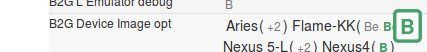
\includegraphics[scale=0.50]{img/treeheder.jpg}
  \end{center}
\end{frame}

\begin{frame}[fragile]{Payload}
  \footnotesize
  \begin{itemize}
    \item Payload is worker specific
    \item Here I am using docker-worker tasks as an example
  \end{itemize}
  \tiny
  \begin{lstlisting}
    payload:
      image: taskclusterprivate/phone-builder:0.0.22
      maxRunTime: 3600

      artifacts:
        private/build:
          expires: '2016-11-26T15:00:22.195275Z'
          path: /home/worker/artifacts/
          type: directory
        public/build:
          expires: '2016-11-26T15:00:22.195331Z'
          path: /home/worker/artifacts-public/
          type: directory

      cache:
        tc-vcs: /home/worker/.tc-vcs

      env:
        GECKO_BASE_REPOSITORY: http://hg.mozilla.org/mozilla-central
        GECKO_HEAD_REF: tip
        GECKO_HEAD_REPOSITORY: http://hg.mozilla.org/mozilla-central
        GECKO_HEAD_REV: tip
  \end{lstlisting}
\end{frame}

\begin{frame}{Branch config}
  \begin{itemize}
    \item Which tasks run on each branch?
    \item \url{taskscluster/tasks/branches}
    \item \url{https://github.com/taskcluster/mozilla-taskcluster/blob/master/src/config/default.yml}
    \item \url{branches/<branch-name>/job_flags.yml}
    \item By default the branch will use \url{branches/base_jobs.yml}
  \end{itemize}
\end{frame}

\begin{frame}[fragile]{Branch config}
  \scriptsize
  \begin{lstlisting}
    builds:
      linux64_gecko:
        platforms:
          - b2g
        types:
          opt:
            task: tasks/builds/b2g_desktop_opt.yml
          debug:
            task: tasks/builds/b2g_desktop_debug.yml
    tests:
      gaia-linter:
        allowed_build_tasks:
          tasks/builds/b2g_desktop_opt.yml:
            task: tasks/tests/b2g_linter.yml
          tasks/builds/mulet_linux.yml:
            task: tasks/tests/mulet_linter.yml
  \end{lstlisting}
\end{frame}

\begin{frame}[fragile]{Running tasks manually}
  \scriptsize
  \begin{lstlisting}
  $ sudo npm install taskcluster-cli -g
  $ ./mach taskcluster-build --owner=wcosta@mozilla.com \
      --head-repository=https://hg.mozilla.org/mozilla-central
      --head-rev=tip \
      tasks/builds/b2g_flame_kk_opt.yml | \
      taskcluster run-task --verbose
  \end{lstlisting}
\end{frame}

\begin{frame}
  \begin{center}
    
\includegraphics[scale=0.30]{img/questions.jpg}
  \end{center}
\end{frame}

\end{document}

